\documentclass[tikz,border=10pt]{standalone}

\usepackage{xcolor}
\usetikzlibrary{
    arrows.meta,
    positioning,
    fit,
    backgrounds
}

\begin{document}

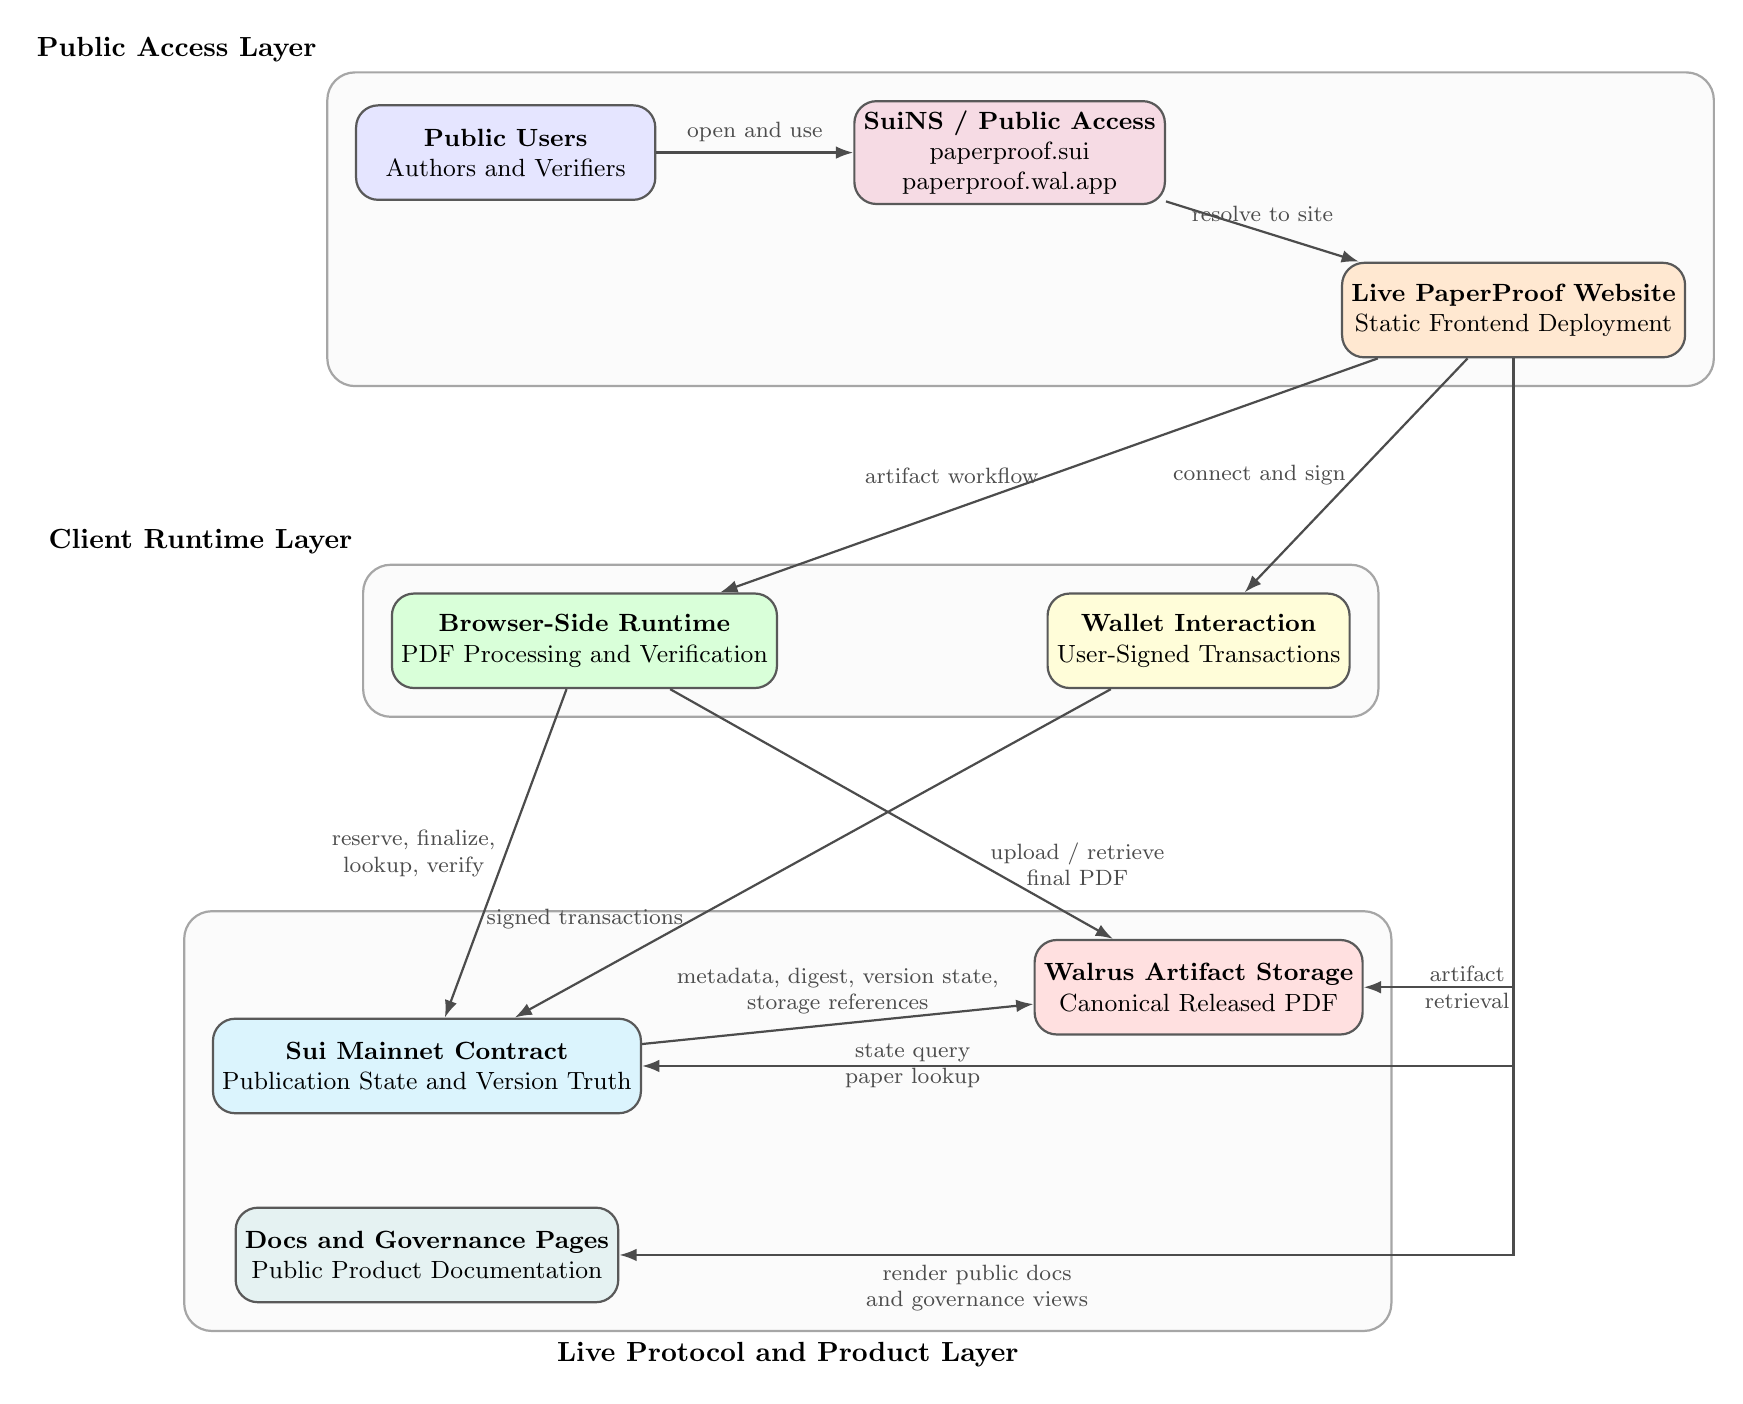
\begin{tikzpicture}[
    font=\small,
    box/.style={
        rectangle,
        rounded corners=8pt,
        draw=black!65,
        thick,
        align=center,
        minimum width=3.8cm,
        minimum height=1.2cm,
        fill=white
    },
    layer/.style={
        rectangle,
        rounded corners=10pt,
        draw=black!35,
        thick,
        fill=gray!3,
        inner sep=10pt
    },
    arrow/.style={
        -{Latex[length=2.2mm,width=1.6mm]},
        thick,
        draw=black!70
    },
    note/.style={
        font=\footnotesize,
        align=center,
        text=black!70
    }
]

% =========================================================
% Public-facing entry
% =========================================================
\node[box, fill=blue!10] (users) at (-2,2)
{\textbf{Public Users}\\Authors and Verifiers};

\node[box, fill=purple!14] (access) at (4.4,2)
{\textbf{SuiNS / Public Access}\\paperproof.sui\\paperproof.wal.app};

\node[box, fill=orange!18] (frontend) at (10.8,0)
{\textbf{Live PaperProof Website}\\Static Frontend Deployment};

% =========================================================
% Local runtime layer
% =========================================================
\node[box, fill=green!15] (browser) at (-1.0,-4.2)
{\textbf{Browser-Side Runtime}\\PDF Processing and Verification};

\node[box, fill=yellow!15] (wallet) at (6.8,-4.2)
{\textbf{Wallet Interaction}\\User-Signed Transactions};

% =========================================================
% Core decentralized backend
% =========================================================
\node[box, fill=cyan!14] (sui) at (-3.0,-9.6)
{\textbf{Sui Mainnet Contract}\\Publication State and Version Truth};

\node[box, fill=red!12] (walrus) at (6.8,-8.6)
{\textbf{Walrus Artifact Storage}\\Canonical Released PDF};

% =========================================================
% Product support surface
% =========================================================
\node[box, fill=teal!10] (docs) at (-3,-12)
{\textbf{Docs and Governance Pages}\\Public Product Documentation};

% =========================================================
% Background layers
% =========================================================
\begin{scope}[on background layer]
\node[layer,
    fit=(users)(access)(frontend),
    label={[font=\bfseries]north west:Public Access Layer}
] {};

\node[layer,
    fit=(browser)(wallet),
    label={[font=\bfseries]north west:Client Runtime Layer}
] {};

\node[layer,
    fit=(docs)(sui)(walrus),
    label={[font=\bfseries]south:Live Protocol and Product Layer}
] {};
\end{scope}

% =========================================================
% Main public access arrows
% =========================================================
\draw[arrow] (users) -- node[above, note] {open and use} (access);
\draw[arrow] (access) -- node[above, note] {resolve to site} (frontend);

% =========================================================
% Frontend runtime arrows
% =========================================================
\draw[arrow] (frontend) -- node[left, note] {artifact workflow} (browser);
\draw[arrow] (frontend) -- node[left, note] {connect and sign} (wallet);
\draw[arrow] (frontend) |- node[pos=0.80, below, note] {render public docs\\and governance views} (docs);

% =========================================================
% Core protocol/storage arrows
% =========================================================
\draw[arrow] (browser) -- node[left, note] {reserve, finalize,\\lookup, verify} (sui);
\draw[arrow] (browser) -- node[pos=0.7, right, note] {upload / retrieve\\final PDF} (walrus);

\draw[arrow] (wallet) -- node[pos=0.7, left, note] {signed transactions} (sui);

\draw[arrow] (sui) -- node[above, note] {metadata, digest, version state,\\storage references} (walrus);

\draw[arrow] (frontend) |- node[pos=0.80, left, note] {state query\\paper lookup} (sui);
\draw[arrow] (frontend) |- node[pos=0.83, right, note] {artifact\\ retrieval} (walrus);

\end{tikzpicture}

\end{document}
